\documentclass[palatino]{epflnotes}

\title{Instability}
\author{Guillermo Julián Moreno}
\date{16/17 - Fall semester}

% Additional packages
\usepackage{tikztools}
\usepackage{caption}
\usepackage{fastbuild}

\usetikzlibrary{shapes}
% --------------------

% \precompileTikz

\begin{document}
\frontmatter
\pagestyle{plain}
\maketitle

\tableofcontents
\mainmatter
% Content

\chapter{Introduction and basic definitions}

\section{Stability}

\begin{defn}[Monotonous stability][Stability!monotonous] A system where, given an initial disturbance of the energy $E$, it tends to the stable state with monotonically decreasing energy function.
\end{defn}

\begin{defn}[Asymptotic stability][Stability!asymptotic] A system where, given an initial energy disturbance, it tends to the stable state with no restrictions on the shape of the function.
\end{defn}

\begin{defn}[Conditional stability][Stability!conditional] A system where the stable state depends of the quantity of the initial disturbance.
\end{defn}

\begin{defn}[Inconditional instability][Instability!inconditional] I don't think this deserves a definition. In some instances we will be interested in small increments of time in order to be able to linearize the equation.
\end{defn}

\section{Case study: dynamical system of a rotating ring}

\begin{figure}[hbtp]
\centering
\inputtikz{RotatingRing}
\caption{A ball in a rotating ring has two different forces: centrifugal and gravity. When the projection of these two are equal, the ball will not move and will thus reach an equilibrum (stable state).}
\label{fig:Introduction:RotatingRing}
\end{figure}

We will study an example of conditional stability: a ball of mass $m$ in a ring of radius $R$ as in \fref{fig:Introduction:RotatingRing}. We want to find the stable state, in which the projections of the centrifugal and gravity forces over the tangent line to the ring cancel themselves.

The gravity force is easy enough: $-mg$ being $g$ the acceleration of gravity. Centrifugal force is easy too: we only have to take into account that the radius at which the ball is rotating (dotted orange path on the figure) depends on the angle θ, simply by $r = R \sin θ$. Thus, the centrifugal force is $mRω^2\cos ω $.

Adding these two forces projected accordingly over the tangent line to the circle (purple line i \fref{fig:Introduction:RotatingRing}) we have the resultant force $F$ exerted over the ball: \( F = -mg\sin θ + mRω^2 \sin θ \cos θ\)

We can substitute the force by the expression $mR\ddot{θ}$ where $\ddot{θ}$ is the angular acceleration of the ball. This gives us the final differential equation for the ball in a rotating ring movement: \( mR\ddot{θ} = -m g \sin θ + m R ω^2 \sin θ \cos θ \label{eq:Introduction:RotatingRingEquationComplete} \)

We can simplify this equation by defining $ω_0^2 = \frac{g}{R}$ as the pendulum frequency, which we will see later why it is interesting. A straightforward substitution yields a simpler equation: \( \ddot{θ} = -ω_0^2 \sin θ + ω^2 \sin θ \cos θ \label{eq:Introduction:RotatingRingEquation} \)

This is not a differential equation that can be solved in a straightforward way. However, we can study what happens when we add a small perturbation.

Our base, stable case is $θ = 0$, which is obviously a solution of \eqref{eq:Introduction:RotatingRingEquation}. What happens when we start with $θ(0) = ε$, with $ε > 0$ as small as required?

Given that ε is small, we can approximate $\sin ε \approx ε$ and $\cos ε \approx 1$ so that our equation becomes \( \ddot{θ} = -ω_0^2 θ + ω^2 θ = (ω^2 - ω_0^2) θ \label{eq:Introduction:RotatingRingSimple} \)

The solution to this simplified differential equation is \( θ = c_1 e^{\sqrt{ω^2 - ω_0^2} t} + c_2 e^{-\sqrt{ω^2 - ω_0^2} t} \label{eq:Introduction:PendulumSolution} \) with $c_1, c_2$ constants depending on the initial conditions. Let's calculate them, as we will need them later to describe the equations. For simplicity, we can suppose that the initial velocity is null ($\dot{θ}(0) = 0$) and thus what we end up with is that $c_1 = c_2 = \sfrac{ε}{2}$

Now on to the actual interesting part: study the behaviour of the solution depending on the value of $ω^2 - ω_0^2$. If $ω^2 < ω_0^2$, the square root is imaginary and our solution will be a cosine: $θ(t) = ε \cos \left[(ω_0^2 - ω^2) t\right]$\footnote{Notice the sign change on $ω_0^2 - ω^2$, important because we want to get the imaginary value out of the square root.}. Thus, in this case the ball will only oscillate between the angles $θ = \pm ε$.

However, if $ω^2 > ω_0^2$, things change. In this case the square root is real, and thus the solution grows exponentially to infinity (first exponential grows, second one quickly decreases to 0 as it has a negative sign). This would be the \textbf{unstable} situation.

An interesting phenomenon is that when we are in the stable zone ($ω^2 < ω_0^2$) but with both quantities very similar, the relaxation time (that is, the time it takes to the system to go back to the stable state) starts to grow up to infinity.

\subsection{Equilibrum states}

\begin{figure}[hbtp]
\inputtikz{RotatingRingStableSolutions}
\caption{Equilibrum points of the rotating ring system with arrows describing whether it's a stable (attracting) or unstable state. The solution $θ_0$ becomes unstable with $\sfrac{ω^2}{ω_0^2} > 1$.}
\label{fig:Introduction:RotatingRingStable}
\end{figure}

Equilibrum states are those that arise as constant functions. Solving \eqref{eq:Introduction:RotatingRingEquation} for $θ = c$ constant, we get first $θ_0 = 0$ and \[ θ_s = \pm \arccos\left(\frac{ω_0^2}{ω^2}\right)\] as solutions, where the latter is only defined for $ω^2 ≥ ω_0^2$. This leads to a bifurcation, as can be seen on \fref{fig:Introduction:RotatingRingStable}.

In order to see that these states are actually stable and not static but unstable points is to see what happens with small perturbations. Thus, we would study the case with initial flow $θ(0) = θ_s \pm εθ'$, and then see what does the solution tend to. I would do it but I don't want to deal with nasty trigonometric calculations, that's for engineers.

After those nasty computations, we would end up with a simplified equation for $θ'$ given by \[ \ddot{θ}' = -θ'ω^2 \sin^2 θ_s \] whose solution is a pure imaginary exponential. That is, we have an stable value.

\chapter{Instabilities}

\section{Rayleigh-Taylor instability}

\begin{figure}[hbtp]
\begin{minipage}[b]{0.45\textwidth}
\centering
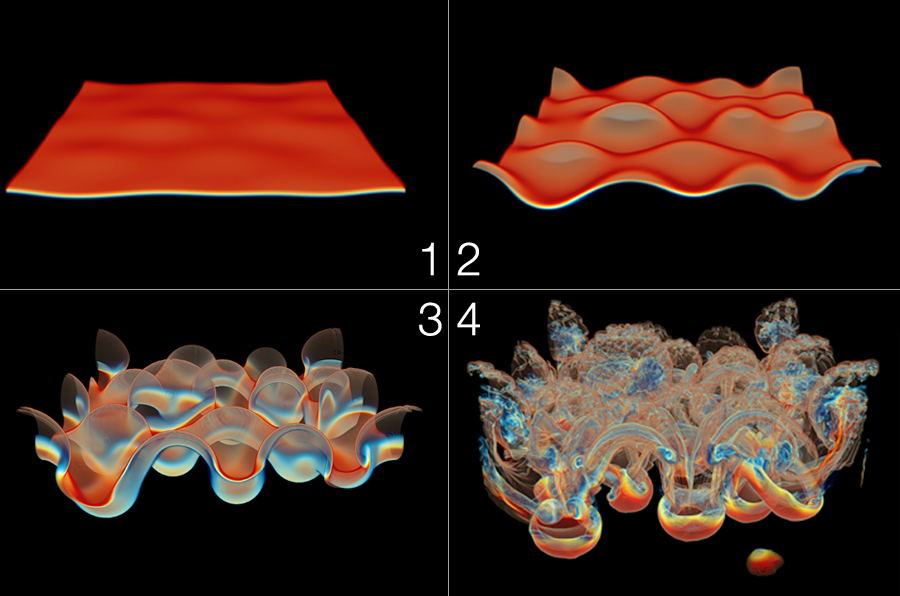
\includegraphics[width=0.8\textwidth]{img/RayleighTaylorInstability.png}
\captionof{figure}{Image of the evolution of the interface with Rayleigh-Taylor instability.}
\label{fig:RayleighTaylorInterfaceImage}
\end{minipage}
\hfill
\begin{minipage}[b]{0.45\textwidth}
\inputtikz{RayleighTaylorModel}
\captionof{figure}{Simplified model of two liquids: 2D and with infinite semiplanes.}
\label{fig:RayleighTaylorModel}
\end{minipage}
\end{figure}

Our first instability will be Rayleigh-Taylor, which models a situation with two impermeable liquids, one below of the other.

To simplify the study of these kind of instabilities, we simplify down to a situation like in \fref{fig:RayleighTaylorModel}. We assume a potential flow with no rotation and no vorticity. Then, to study it we will follow the steps outlined previously.

\subsection{Equations and boundary conditions}

Our potential flow is $ΔΦ_1 = ΔΦ_2 = 0$, so our velocity equations are \begin{align*}
U_1 &= \dpd{Φ_1}{x} & V_1 = \dpd{Φ_1}{z} \\
U_2 &= \dpd{Φ_2}{x} & V_2 = \dpd{Φ_2}{z}
\end{align*}

The velocities $U$ represent the movement of the flow parallel to the $x$ axis, and $V$ represents the velocity parallel to the $z$ axis.

The boundary conditions will be zero values for $Φ_1$ and $Φ_2$ at $z = \mp ∞$ respectively: we don't want the flows to move at infinity.

\begin{figure}
\centering
\inputtikz{RayleighTaylorInterface}
\caption{Interface η in Rayleigh-Taylor instability.}
\label{fig:RayleighTaylorInterface}
\end{figure}

The next step is the definition of the interface, the set of points where the two flows ``touch'', and define the relations at that boundary. The first condition is that of impermeability: no particles pass through the interface. That means that whatever displacement $δη_\perp$ of the interface in its normal direction must be caused by the velocity of the flow. On one hand, our displacement is $δη_\perp = ∂η_t \cos α$. On the other, we have two sources of velocity of the flow: the vertical movement $V_1$ and the horizontal $U_1$. For both of them we will calculate their projection normal to the interface at any point. Thus, we will have
\begin{align}
δη_\perp &= V_\perp - U_\perp \nonumber \\
\dpd{η}{t} \cos α &= V_1 \cos α - U_1 \sin α \nonumber \\
\dpd{η}{t} &= V_1 - U_1 \tan α \nonumber \\
\dpd{η}{t} &= V_1 - U_1 \dpd{η}{x} \label{eq:RayleighTaylor:KinematicConds}
\end{align}

We will have analogous equations for the second fluid.

Now we have to define the dynamic boundary conditions, the ones that relate the interface to the difference of pressure between the two fluids.

Our kinematic condition is that we will force impermeability, so that normal components to the interface must be equal. Now for the fluid we write down some equations and something.

Now on to the dynamic boundary conditions. Using Laplace's law for pressure % TODO: Write it
which tells us that $P_1 - P_2 = γ\frac{2}{R}$, with γ the surface tension and $R$ the radius of curvature. Thus, our condition at $z = η$ \( P_1 - P_2 = -γ \frac{\dpd[2]{η}{x}}{\left(1 + \left(\pd{η}{x}\right)^2 \right)^{\sfrac{3}{2}}} \label{eq:RayleighTaylor:DynamicConds} \)

Finally, we have the Bernouilli's principle to tie everything up:

\begin{align}
\dpd{Φ_1}{t} + \frac{U_1^2 + V_1^2}{2} + \frac{P_1}{ρ_1} + gz &= C_1(t) \label{eq:RayleighTaylor:Bernoulli} \\
\dpd{Φ_2}{t} + \frac{U_2^2 + V_2^2}{2} + \frac{P_2}{ρ_2} + gz &= C_2(t)
\end{align}

Looking at these relations at infinity, we assume that nothing changes there so we can equate $C_1(t) = C_2(t) = 0$ and life is easier. Putting everything together, our equations defining the base state of the system are the following:

\begin{align*}
0&= Φ_1(∞) & 0&= Φ_2(-∞) \\
U_1 &= \dpd{Φ_1}{x} & U_2 &= \dpd{Φ_2}{x} \\
V_1 &= \dpd{Φ_1}{z} & V_2 &= \dpd{Φ_2}{z} \\
\dpd{η}{t} &= V_1 - U_1 \dpd{η}{x} & \dpd{η}{t} &= V_2 - U_2 \dpd{η}{x} \\
0 &= \dpd{Φ_1}{t} + \frac{U_1^2 + V_1^2}{2} + \frac{P_1}{ρ_1} + gz &
	0 &= \dpd{Φ_2}{t} + \frac{U_2^2 + V_2^2}{2} + \frac{P_2}{ρ_2} + gz \\
\end{align*}
\vspace{-30pt}
\[ P_1 - P_2 = -γ \frac{\dpd[2]{η}{x}}{\left(1 + \left(\pd{η}{x}\right)^2 \right)^{\sfrac{3}{2}}} \]

\subsection{Small perturbation and linearization}

To study what happens, we add small perturbations $εφ_1$ and $εφ_2$ to the flows (maintaining $φ_1 = φ_2 = 0$ at $\pm ∞$ respectively), $εp_1$, $εp_2$ to the pressure and $εσ$ to the interface displacement, with $ε \ll 1$; and we study what happens. For the kinematic conditions \eqref{eq:RayleighTaylor:KinematicConds}, we will see that the perturbation follows the equation \[ ε \pd{σ}{t} = εv_1 - ε^2 u_1 \pd{σ}{x} \] with $v_1 = ∂_z φ_1$, $u_1 = ∂_x φ_1$. Given that ε is small, we can ignore the quadratric term so we have the following equations: \[ v_1 = v_2 = \pd{σ}{t} \text{ at } z = εσ  \]

We have a small problem there with the fact that we don't know where the interface is. However, as ε is small, we can do Taylor expansion\footnote{No we can't as we don't have absolutely any regularity conditions assured. But this is not a mathematics course.} and set the interface at $z = 0$, with equations \( v_1 = v_2 = \pd{φ_1}{z} = \pd{φ_2}{z} = \pd{σ}{t} \text{ at } z = 0 \label{eq:RayleighTaylor:KinematicBoundaryLineareized} \)

We do the same process with the dynamic conditions \eqref{eq:RayleighTaylor:DynamicConds}. The equations of the perturbation are \[ \eval{\left(P_1 + εp_1 -P_2 - εp_2\right)}_{εσ} = -γ ε \dpd[2]{σ}{x} \left(1 - \frac{3}{2}ε^2 \left(\dpd{σ}{x}\right)^2 \right)\] and replacing $P_1 = -gρ_1 z$ and linearizing and flattening (setting the interface at $z = 0$) we end up with \( (ρ_2 - ρ_1)gσ + \eval{(p_1 - p_2)}_{0} = - γ\dpd[2]{σ}{x} \label{eq:RayleighTaylor:BernoulliLinearized} \)

Finally, doing the same with the Bernouilli relations \eqref{eq:RayleighTaylor:Bernoulli} (I'm not copying the computations again) we have \( \dpd{φ_1}{t} + \frac{p_1}{ρ_1} = 0 \qquad  \dpd{φ_2}{t} + \frac{p_2}{ρ_2} = 0 \label{eq:RayleighTaylor:Pressure} \)

\subsection{Normal mode analysis}

Given that the previous equations do not seem easy to solve analytically, we do some magic handwaving called normal mode analysis. With this, we assume that the solution is going to present periodical behaviour in $x$ and $t$, with an excitation depending on $z$. Assume the frequencies of these two excitations are $k$ and ω (notation: wavenumber and frequency), we would then have the following equations: \(
\begin{cases}
φ_1 = f_1(z)e^{\imath (kx - ωt)} \\
φ_2 = f_2(z)e^{\imath (kx - ωt)} \\
σ = C e^{\imath (kx - ωt)}
\end{cases} \label{eq:RayleighTaylor:Solutions}
\)

In order to obtain the equations of $f_1$ and $f_2$, we use the fact that the flow has to be potential, so $Δφ_1 = 0$. From that, we start solving:
\begin{align*}
\dpd[2]{φ_1}{x} + \dpd[2]{φ_1}{z} &= 0 \\
\imath^2 k^2 f_1(z) e^{\imath (kx - ωt)} + f_1''(z) e^{\imath (kx - ωt)} &= 0 \\
f_1''(z) = k^2 f_1(z)
\end{align*}

This is a second-order differential equation with general solution $f_1(z) = A_1 e^{kz} + A_2 e^{-kz}$, and we would obtain an analogous result $f_2(z) = B_1 e^{kz} + B_2e^{-kz}$ for $φ_2$. With that, we can replace in the boundary conditions:
\begin{align}
φ_1(-∞) = 0 &\implies A_2 = 0  \label{eq:RayleighTaylor:AppliedBoundary1} \\
φ_2(∞) = 0 &\implies B_1 = 0 \label{eq:RayleighTaylor:AppliedBoundary2}
\end{align}

So we can assume that $f_1(z) = Ae^{kz}$ and $f_2(z) = Be^{-kz}$ for some constants $A, B ∈ ℝ$. Replacing these solutions in the linearized equations, we end up with \begin{align*}
g(ρ_2 - ρ_1)C + \imath ωρ_1A - \imath ω ρ_2 B &= γk^2 C \\
kA &= -\imath ω C \\
- kB &= -\imath ω C
\end{align*} which we can solve for $ω$ multiplying by $k$ and replacing $k A$ and $kB$:
\begin{align}
kg(ρ_2 - ρ_1)C + ω^2 ρ_1 C + ω^2 ρ_2 C &= γk^3 C \nonumber \\
ω^2 =\frac{-kg(ρ_2 - ρ_1) + γk^3 }{ρ_1 + ρ_2}
\end{align}

\subsection{Stability analysis}

This is enough to do a quantitative analysis. If $\Im ω > 0$, in our flows $φ_1, φ_2$ we will have an exponential like $e^{\imath (- \imath \Im ω)} = e^{\Im ω}$, a positive exponential that will diverge, and thus we will have an unstable flow. The other possibility is that we have $\Im ω = 0$, in which case we would have oscillating solutions (imaginary exponential). The case $\Im ω < 0$ is not possible in this case, but if it were we would have a damped solution. These types of solutions appear when viscosity is not ignored.

\begin{figure}[hbtp]
\inputtikz{RayleighTaylorStability}
\caption{Imaginary value of the frequency $\Im ω$ in the Rayleigh-Taylor interface, depending on the the value $\frac{1}{λl_c}$, with $l_c$ the capillary length and $λ$ the wavelength. Red zones are unstable, green zones are stable. The dashed lines represent the case with damping, which is not possible with the simplficiations we have made.}
\label{fig:RayleighTaylor:Stability}
\end{figure}

What is interesting is that the stability depends on the fluid density. If $ρ_1 > ρ_2$ (that is, the denser fluid is below) then $ω^2$ is always positive and the solutions are oscillations. If $ρ_2 > ρ_1$ (denser fluid above), the unstable case may appear depending on the wavenumber, the pressure difference and the surface tension. We can, in fact, combine those three values in the capillary length, given by \[ l_c = \sqrt{\frac{γ}{g\abs{ρ_2 - ρ_1}}} \] which tells us the point at which capillary and gravity forces are in equilibrum.

\subsection{Specific cases without semi-infinite planes}

\begin{wrapfigure}[13]{R}{0.25\textwidth}
\centering
\inputtikz{RayleighTaylorClosed}
\caption{Rayleigh-Taylor instability in a cube.}
\label{fig:RayleighTaylorClosed}
\end{wrapfigure}

Until now, we have been assuming that our fluids have an infinite interface. What happens when we consider fluids on a limited space, or even in a cube (\fref{fig:RayleighTaylorClosed})?

In the case of a limited space, the boundary conditions just restrict the possible wavelengths, as they must be divisors of the length of the boundary. For example, if the length of the opening is $l$, then the only possible wavelengths are $\sfrac{l}{n}$ for $n ∈ ℕ$. If the opening is smaller than the capillary length, we are in a stable situation (e.g., when we put a small tube filled with water facing down). If the opening is too big, some wavelengths will be in the unstable region, so we will be in an unstable case and the fluid will fall.

In the case of the cube, it would be a little bit more complicated because of the expression of curvature in 2D. However, instead of doing the Fourier transform we would do the Fourier series expansion (finite domain) and then study the discretized dispersion relation. The Fourier basis used should be based on sinus, as those can be made 0 at the boundaries which is probably our desired conditions.

\subsection{Dispersion relation for water waves: Gravito-capillary waves}
\label{sec:RayleighTaylor:WaterWaves}
\label{sec:GravitoCapillary}

\begin{figure}[hbtp]
\centering
\inputtikz{WaterWaves}
\caption{Waves in the ocean, modeled as a Rayleigh-Taylor instability (fluid above is air) with a limited second fluid of height $H$.}
\label{fig:RayleighTaylor:WaterWaves}
\end{figure}

One interesting study is to see what happens in water waves, where instead of having an infinite plane we have a plane of height $H$ (\fref{fig:RayleighTaylor:WaterWaves}). For simplification, the fluid above is not important so we can set $ρ_2 = 0$ and ignore it in the calculations.

The limited height changes the boundary conditions. Now we want to ensure that $\eval[0]{∂_z φ_1}_{z = -H} = 0$, that is, that the fluid doesn't move vertically at the bottom of the ocean. Doing the appropriate calculations, we have \begin{align*}
\eval{\dpd{φ_1}{z}}_{z = 0} &= 0 \\
\left(kA_1 e^{-kH} -k A_2e^{kH}\right) e^{\imath (kx - ωt)} &= 0 \\
A_1e^{-kH} - A_2e^{kH} &= 0 \\
A_1 = A_2 e^{2kH}
\end{align*}

Now we repeat the same process as before. First, we obtain the relation from the linearized  kinematic boundary condition at $z = 0$ \eqref{eq:RayleighTaylor:KinematicBoundaryLineareized}, remembering that the solution for $σ$ was $σ = Ce^{\imath (kx - ωt)}$ \eqref{eq:RayleighTaylor:Solutions}: \begin{align*}
\dpd{φ_1}{z} &= \dpd{σ}{t} \\
\eval[1]{(A_1 ke^{kz} - A_2 ke^{-kz})e^{\imath (kx - ωt)}}_{z = 0} &= -\imath ω C e^{\imath (kx - ωt)} \\
A_1 - A_2 &= -\frac{\imath ω C}{k} \\
A_2(e^{2kH} - 1) &= -\frac{\imath ω C}{k} \\
A_2 &= - \frac{\imath ω C}{k(e^{2kH} - 1)}
\end{align*}

With \eqref{eq:RayleighTaylor:Pressure} we can obtain the pressure as an expression of the flow \[ p_1 = - ρ_1 \dpd{φ_1}{t} = ρ_1 \imath ω φ_1  \] and then finally put everything together replacing appropriately in \eqref{eq:RayleighTaylor:BernoulliLinearized} (remembering also that $p_2 = ρ_2 = 0$): \begin{align*}
- ρ_1gσ + \eval[1]{p_1}_{z=0} &= - γ\dpd[2]{σ}{x} \\
- ρ_1 g C e^{\imath (kx - ωt)} + \eval[0]{ρ_1 \imath ω φ_1}_{z = 0} &= -γ\imath^2 k^2 σ \\
- ρ_1 g C e^{\imath (kx - ωt)} + \eval[1]{ρ_1 \imath ω (A_1 e^{kz} + A_2 e^{-kz}) e^{\imath (kx - ωt)}}_{z = 0} &= γk^2 C e^{\imath (kx - ωt)} \\
- ρ_1 g C + ρ_1 \imath ω (A_1 + A_2) &= γk^2 C \\
- ρ_1 g C + ρ_1 \imath ω A_2(e^{2kH} + 1) &= γk^2 C \\
- ρ_1 g C + ρ_1 \imath ω \frac{- \imath ω C}{k(e^{2kH} - 1)}(e^{2kH} + 1) &= γk^2 C \\
ω^2 = \left(\frac{γk^3}{ρ} + ρ_1 k\right) ·  \frac{e^{2kH} - 1}{e^{2kH} + 1}
\end{align*}

Finally, knowing that $\tanh x = \frac{e^{2x} - 1}{e^{2x} + 1}$, the dispersion relation is \( \boxed{ω^2 = \left(\frac{γk^3}{ρ} + gk\right) \tanh kH}  \)

In that case, our capillary wave number is $k_c = \sqrt{\sfrac{ρg}{γ}}$, and we can scale our length, time scale and the parameter depending on the height: \begin{align*}
\tilde{k} &= \frac{k}{k_c} \\
\tilde{ω} &= \frac{ω}{k_c} \\
\tilde{H} &= Hk_c \\
\end{align*}

\begin{table}[hbtp]
\centering
\begin{tabular}{cc|c|c}
& & Gravity & Capillary \\
& & $\tilde{k} \ll 1$ & $\tilde{k} \gg 1$ \\ \toprule
Shallow water & $\tilde{k} \ll \sfrac{1}{\tilde{H}}$ & $ω = $ & $ω = $ \\ \midrule
Deep water & $\tilde{k} \ll \sfrac{1}{\tilde{H}}$ & $ω = $  & $ω = $ \\ \bottomrule
\end{tabular}
\caption{Values of ω depending on the situation of the waves}
\label{tab:RayleighTaylorWater}
\end{table}

With that, we can find the value of $ω$ depending on whether we are on shallow or deep water, and on whether it is more important gravity or capillarity, as we can see in \fref{tab:RayleighTaylorWater}.

This makes an important difference in how the waves behave. For example, we can study the group and phase velocity of the waves in the ocean. So I paste here the graphic.

\section{Rayleigh-Plateau instability}
\label{sec:RayleighPlateau}

\begin{figure}[hbtp]
\centering
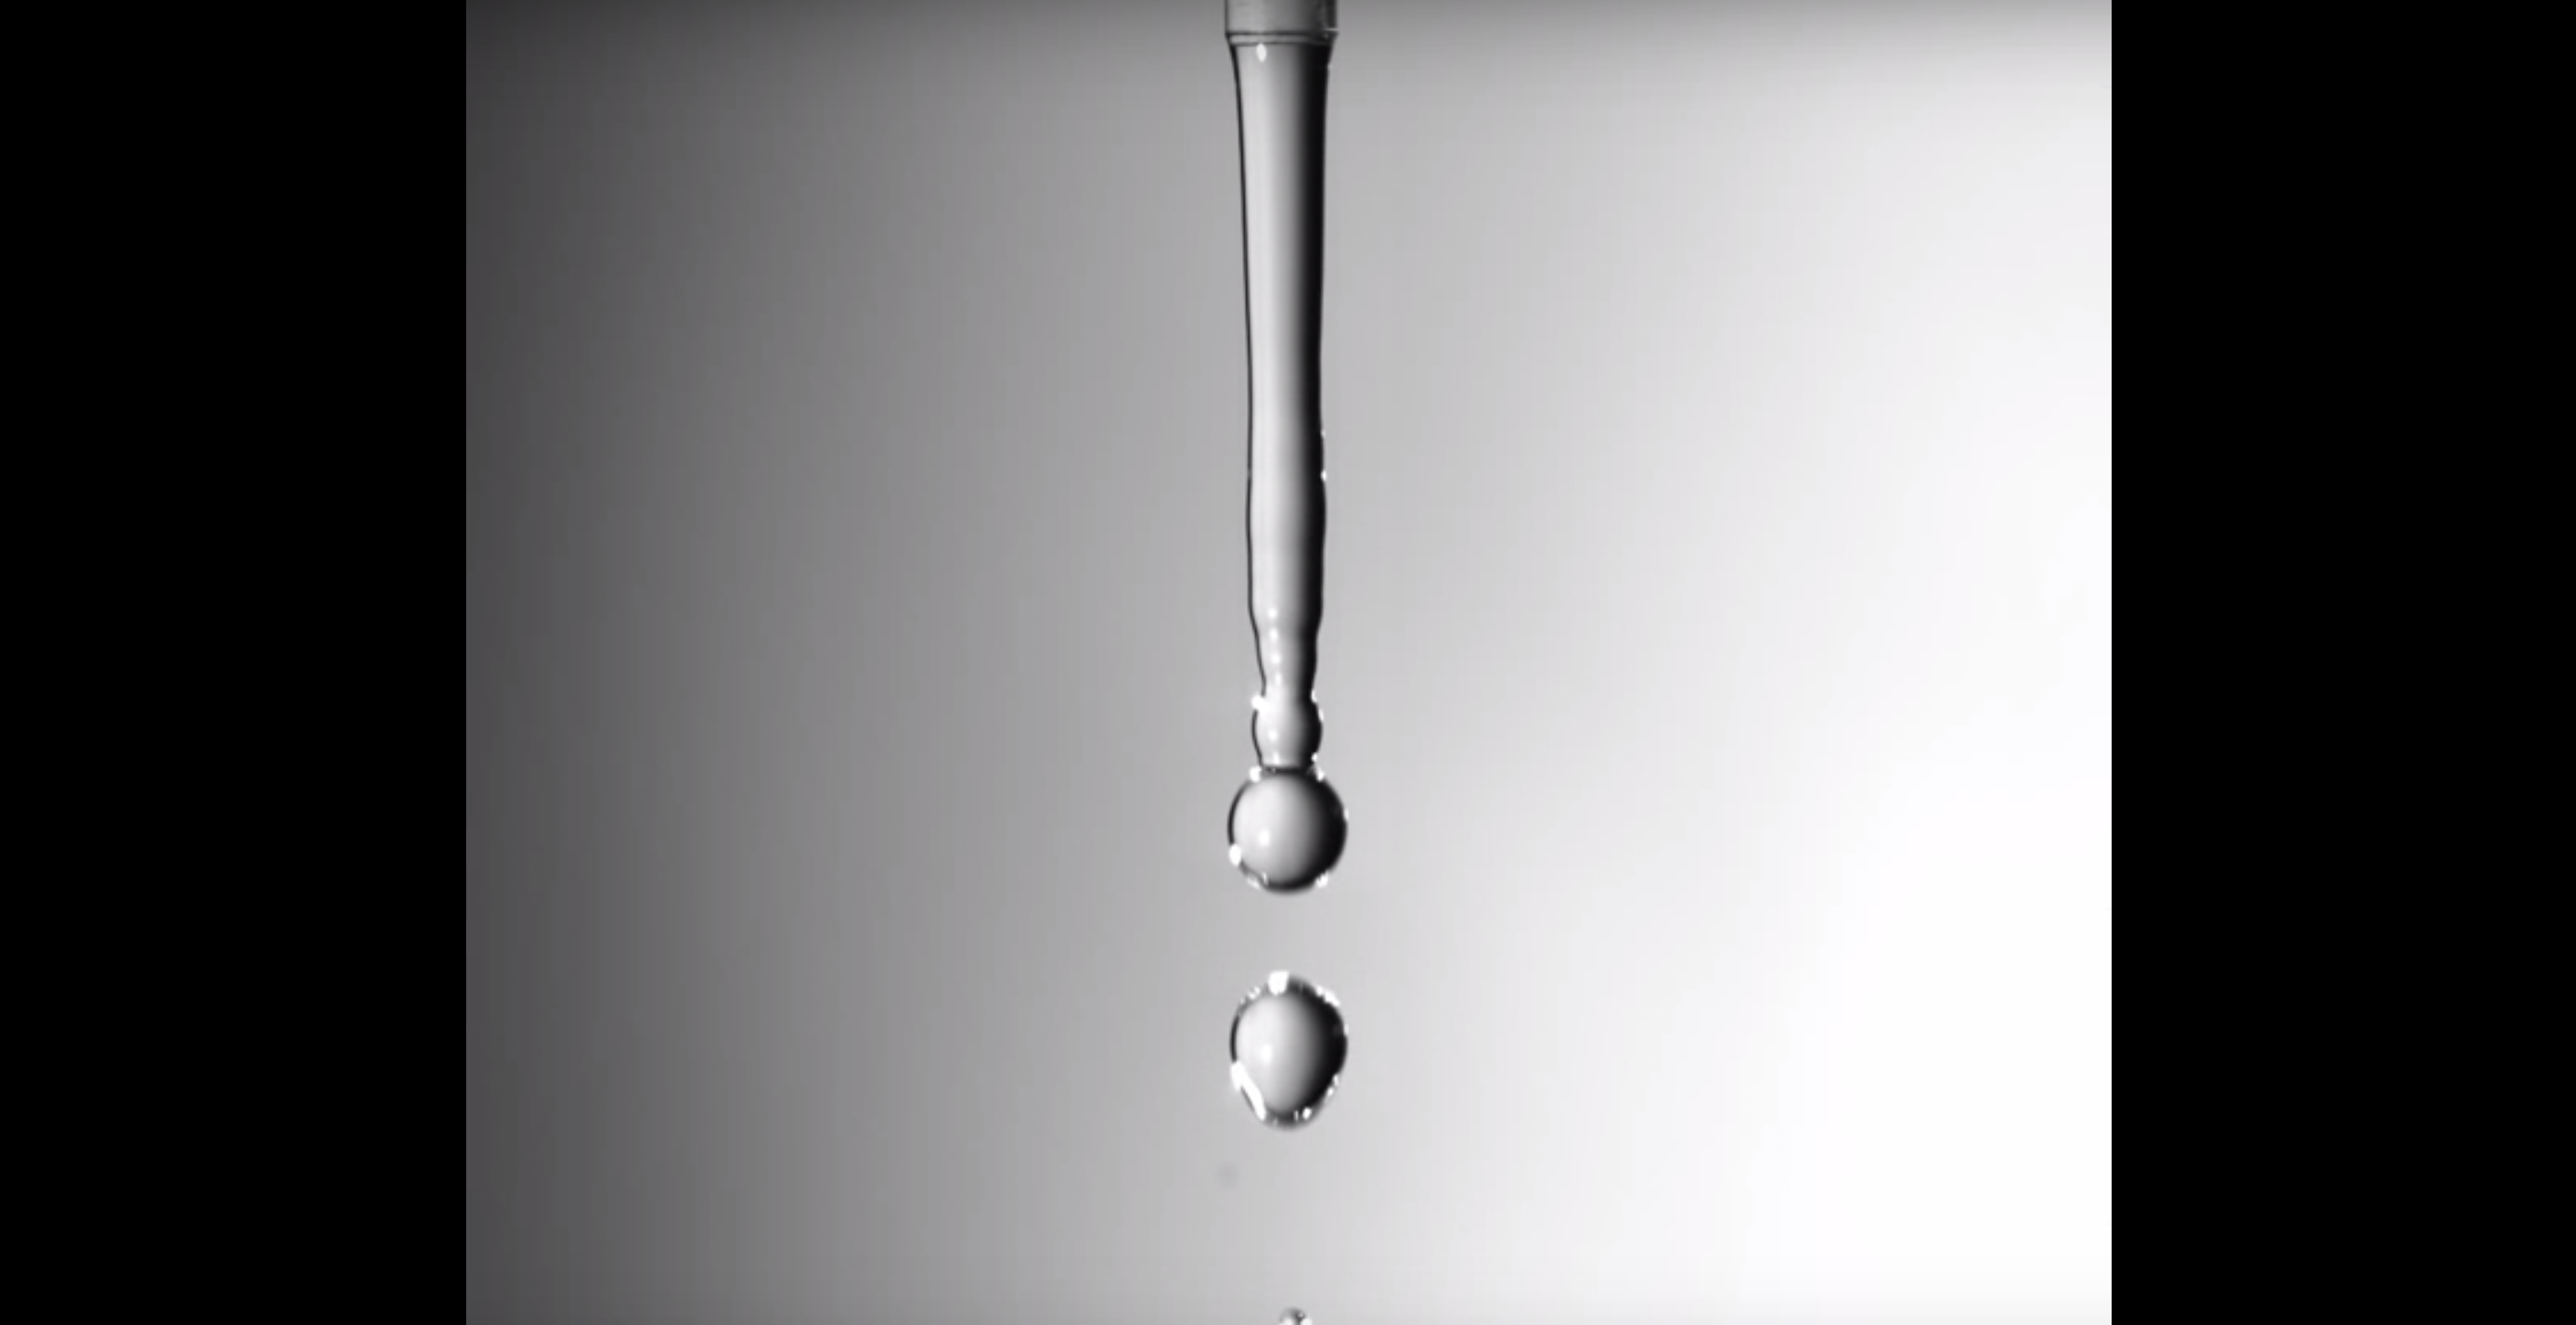
\includegraphics[width=0.8\textwidth]{img/RayleighPlateauInstability.png}
\caption{Rayleigh-Plateau instability: A jet that forms droplets.}
\label{fig:RayleighPlateau:Jet}
\end{figure}

The next instability to study is Rayleigh-Plateau, which models the instability in a cylindrical jet such as in \fref{fig:RayleighPlateau:Jet}.

\begin{wrapfigure}[13]{R}{0.4\textwidth}
\centering
\inputtikz{CylinderSpheres}
\caption{Two possible configurations: A cylindrical jet or $n$ spheres.}
\end{wrapfigure}

In this type of instability, the driving force is surface tension. We have two possible configurations: a cylindrical tube of radius $R$ or a set of $n$ spheres of radius $a$. For a fixed volume $V$, surface tension will tend to force the configuration with less surface area.

Fixing the volume gives us the number of necessary spheres for fixed radius $a$, $R$: \[ πR^2 h = n\frac{4}{3} πa^3 \implies n = \frac{3R^2 a^3}{4} \]

Then, supposing that $h \gg R$, we can ignore the ``caps'' of the cylinder and find for which values of $a, R$ we have less surface on the sphere configuration:
\begin{align*}
2πRh &< n4πa^2 \\
2πRh &< \frac{3R^2 a^3}{4} 4πa^2 \\
\end{align*}

We can move also to a dynamical analysis. The Laplace law tells us the relation between pressure of the water, surface tension γ, curvature ζ and atmospheric pressure: \( P_{\text{water}} = P_{\text{atm}} + γζ \)

The base state, the flow without perturbation, has equation $P_0 - P_{\text{atm}} = \frac{γ}{R_0}$. In a crest and in a valley of the flow, we will have different radius $R_c = R_0 + δR$, $R_v = R_0 - δR$ respectively with $δR > 0$. That gives us two different equations for those two points
\begin{align*}
P_c - P_{\text{atm}} &= \frac{γ}{R_0} \left(1 - \frac{δR}{R_0}\right) \\
P_v - P_{\text{atm}} &= \frac{γ}{R_0} \left(1 + \frac{δR}{R_0}\right)
\end{align*}
which in turn tells us that $P_v > P_c$.

This is important, because Bernouilli law tells us that flow moves from high to low pressure zone. That will force more water in the `crest' zone which will make the flow more unstable.

\subsection{Equations and boundary conditions}

Once we have made the handwaving argument to see how the flow should behave, we can start doing the instability analysis. The base equations are the Navier-Stokes equations in cylindrical geometry. Those are pretty complex, but one can start doing simplifications neglecting viscosity and gravity, and assuming a flow symmetric and without swirl around the axis.

Then, our simplified equations are (TODO:Fix them) \begin{align}
\dpd{u_r}{t} + U \dpd{u_r}{z} &= - \frac{1}{ρ} \dpd{p}{r} \label{eq:RayleighPlateau:EulerR}\\
\dpd{u_z}{t} + U \dpd{u_z}{z} &= - \frac{1}{ρ} \dpd{p}{z} \label{eq:RayleighPlateau:EulerZ}\\
\frac{1}{t} \dpd{(ru_r)}{r} + \dpd{u_z}{z} &= 0 \label{eq:RayleighPlateau:EulerP}
\end{align}

The kinematic boundary conditions are derived in the same fashion that we did with the Rayleigh-Taylor instability (\fref{fig:RayleighTaylorInterface}), which gives us an equation for the interface $R$: \( \dpd{R}{t} = u_r - u_z \dpd{R}{z} \label{eq:RayleighPlateau:Interface} \)

For the dynamic boundary conditions, we do some awful computations and then end up with a more awful thing.

\subsection{Base flow, perturbation and linearization}

The base flow is very easy, which is just a cylindrical flow with interface $R(x,t) = R_0$, and pressure $P_0 = P_{\text{atm}} + \sfrac{γ}{R_0}$. It is easy to check that it is actually a solution of the equations we wrote previously.

Now we study what happens when we add a small perturbation: $U_r = ε u_r$, $U_z = U_0 + εu_z$, $P = P_0 + εp$. We replace that in the Euler equation for the $z$ axis and neglect the terms with $ε^2$ as those will not be very important
\begin{align*}
\dpd{U_z}{t} + U_r \dpd{U_z}{t} + U_z \dpd{U_z}{z} &= - \dpd{P}{z} \\
ε\dpd{u_z}{t} + ε^2u_r \dpd{u_z}{t} + U_0 ε \dpd{u_z}{z} + ε^2u_z \dpd{u_z}{z} &= - ε\dpd{p}{z} \\
\dpd{u_r}{t} + U_0 \dpd{u_z}{z} &= - \dpd{p}{z}
\end{align*}

Doing that with all the equations \eqref{eq:RayleighPlateau:EulerR,eq:RayleighPlateau:EulerZ,eq:RayleighPlateau:EulerP} we end up with
\begin{align}
\dpd{u_r}{t} + U \dpd{u_r}{z} &= - \frac{1}{ρ} \dpd{p}{r} \\
\dpd{u_z}{t} + U \dpd{u_z}{z} &= - \frac{1}{ρ} \dpd{p}{z} \\
\frac{1}{t} \dpd{(ru_r)}{r} + \dpd{u_z}{z} &= 0
\end{align} which we can simplify doing ugly manipulations to a single equation \( \label{eq:RayleighPlateau:SingleSolution} \)

Perturbing and linearizing the boundary conditions we end up with another thing. I'm going to copy this later.

\section{Kelvin-Helmholtz instability}

Two interpretations, Bernoulli and rotation, see slides. Then use Euler equations (incompressible Navier-Stokes without viscosity), and we need to force continuity with $∂_xu + ∂_y v = 0$ so usnig the streamfunctions gives is this condition for free.

\[ u = ∂_y ψ \quad v = ∂_x ψ \]

Things similar to Rayleigh-Taylor. Key in other instabilities, and inflection points.

\section{Cylinder wake}

Two-dimensional instability.

About parallel flows: for any given 3D instability we can find another 2D instability with lower reynolds number.

\section{Vorticity?}

Sinous, varicose and single street flows: vorticity sheets turning into discrete vortices.

Inviscid limitt! We take euler equations
\begin{align*}
\dpd{\vu}{t} + \vu \grad \vu &= - \grad p \\
\dv \vu &= 0
\end{align*} which are Navier-Stokes without viscosity and incompressible fluid ($\dv u = 0$).

Our base flow is $\vu = u(y) \ve_x$. Then we add a perturbation $u'$.  Equations, things, calculations. Then linearized euler. Then more computations and details, normal mode expansion because there's no deependence between $x, z, t$ so wavenumbers are independent. Final equations (hats are Fourier transforms:
\begin{align*}
- \imath ω\hat{u}_x + U(y) \imath k_x \hat{u}_x + \hat{u} \dod{U(y)}{y} &= - \imath k_x \hat{p} \\
-\imath ω \hat{u}_y + U(y) \imath k_x \hat{u}_y + 0 &= - \dpd{\hat{p}}{y} \\
-\imath ω \hat{u}_z + U(y) \imath k_x\hat{u}_z &= -i k_z \hat{p} \\
\imath k_x \hat{u}_x + \dod{\hat{u}_y}{y} + \imath k_z \hat{u}_z &= 0 \end{align*}

The last one is the divergence of the Fourier expansion. Once here, we do a transformation $\tilde{k} = \sqrt{k_x^2 + k_z^2}$ which is in the slides. Even more horrible equations

I don'tknow how but non-orthogonality of the eigenvalues may imply a transient growth of the isntability which in turn may cause instability even in asymptotically stable states. Very cool. Operator norms and singular value decompositions.

\appendix

\chapter{Exercises}
% -*- root: ../Instability.tex -*-
\section{Instability of a thin suspended film}

Something something.


\chapter{Other data about the subject}

Exam will be a presentation of a paper, and then a small 20 \% written exam. The papers are the following:

\begin{enumerate}
	\item Rayleigh-Taylor in thin cell. They use magnetic levitation to create the base stable flow. The flow is parabolic in the direction of the depth.
	\item Rayleigh-Taylor under an incline. Same problem of the ``thin layer'' of the first exercise but tilting the plane.
	\item Saffmann-Taylor instability (the fingers one). 25 pages.
	\item Rayleigh-Plateau instability of co-flowing viscous jets.
	\item Influence of confinement on vortex shedding. Explanation of vorticity appearing. Feasible case of numerics.
	\item Stability analysis on mean flow. They average the flow or something. Sounds interesting.
	\item Convective instability behind a cylinder. Similar to the previous one.
	\item Shear-flow instability in circular geometry.
	\item Rayleigh-Benard-Poiseuille which is Rayleigh-Benard with advection.
	\item Transient growth in Rayleigh-Benard-Poiseuille.
	\item Pearls on a fiber.
	\item Viscous effects in Rayleigh-Taylor instability.
	\item Draw resonance.
	\item Dry friction on the bead on a hoop.
\end{enumerate}



\backmatter
\printindex
\end{document}
